\section{Project management}
\label{section:project_management}

We present herein a discussion of all deviations from the initial project constraints concerning its management.

\subsection{Scope}
\label{section:scope}

\subsubsection{Requirements analysis}

There have been no major changes in the scope of the project. Both the functional and non-functional requirements sets remain the same as the ones defined in the final report of the Project Management course.

We provide now a summary of the current state of the project, in terms of what requirements have already been fulfilled throughout its development phase (see the Schedule section~\ref{section:schedule}):

\begin{itemize}
	\item \textbf{Functional requirements:} 
	\begin{enumerate}
		\item \textbf{[In Progress]} Implement privacy preserving stream mining \textit{filters} for the MOA stream mining framework. The suggested algorithms to be implemented are:
		\begin{enumerate}
			\item \textbf{[Completed]} Noise addition~\cite[p.~54]{book:StatisticalDisclosureControl}
			\item \textbf{[Not started]} Multiplicative noise~\cite[p.~57]{book:StatisticalDisclosureControl}
			\item \textbf{[Completed]} Microaggregation~\cite[p.~60]{book:StatisticalDisclosureControl}
			\item \textbf{[Completed]} Rank swapping~\cite[p.~72]{book:StatisticalDisclosureControl}
			\item \textbf{[Not started]} Rank shuffling~\cite[p.~73]{book:StatisticalDisclosureControl}
			\item \textbf{[Not started]} Differential privacy~\cite{Dwork06differentialprivacy}
		\end{enumerate}
	\end{enumerate}
\end{itemize}

Concerning the non-functional requirements of the project, there are some of them that should be emphasized from now on, in order to correctly achieve them at the end of the development phase.

\begin{itemize}
	\item \textbf{Non-functional requirements to be emphasized:}
	\begin{enumerate}
		\item \textbf{Test coverage:} measures and tests will be performed to assess the quality of the developed software, as well as its scalability and performance, which is paramount in this project’s context.
		\item \textbf{Documentation:} MOA is an \textit{open source} data mining framework, which means that its community can assess how is it built and how to improve it. One of the benefits of the open source development model is that software can be safer, more robust and efficient, by receiving contributions from different developers. If people are to continue improving the work done, it has to be well documented.
	\end{enumerate}
\end{itemize}

\subsubsection{Methodology}

Even though no significant changes have been made to the methodological framework being used, an agreement has been reached to apply it \textit{more rigorously}, in order to enhance the project monitoring and to avoid further schedule deviations.

In this respect, the usage of the Trello\footnote{Available at: \url{https://trello.com/}} task management system will be emphasized from now on, as it provides all necessary features to overcome the detected methodological errors.

\subsection{Schedule}
\label{section:schedule}

There have been significant deviations concerning the initial project schedule. Not only the global duration has been lengthened, but more phases have been layed out, as was needed. As a positive contrast, early detection of such alterations has been sometimes possible.

\subsubsection{Overall duration}

The original total duration has been extended from 5 months to 8 months, approximately. Thus, the final report and its defence is now scheduled to be in April, which is the next available lecture shift in the Faculty. We believe that this extended duration will allow us to fulfill all requirements defined in the scope of the project.

\subsubsection{Deviation analysis}

There are several possible reasons behind this schedule deviation:

\begin{itemize}
	\item The Project Management module lasted longer than expected, forcing the development phase of the project to begin later.
	\item During the definition of the project initial schedule, we expected to begin developing it while the Project Management module endured, which was, definitely, a planning error. Such tasks concurrency was not possible at that time.
	\item At the beginning of the development phase, we explored different technological alternatives, before deciding which approach was mostly suited to our needs, but this exploration delayed the actual development process for a couple of weeks.
	\item As was already stated in the Project Management report, some of the requested features have posed to be more complicated than was expected, consuming some more time than that assigned to them.
	\item For personal reasons, no work could be carried out during the Christmas vacations, which lasted two more weeks, furtherly delaying the project's development.
\end{itemize}

\subsubsection{Current detailed schedule}

Considering the previous analysis, a new Gantt chart has been built, with the new project's schedule, which is detailed in the following pages.

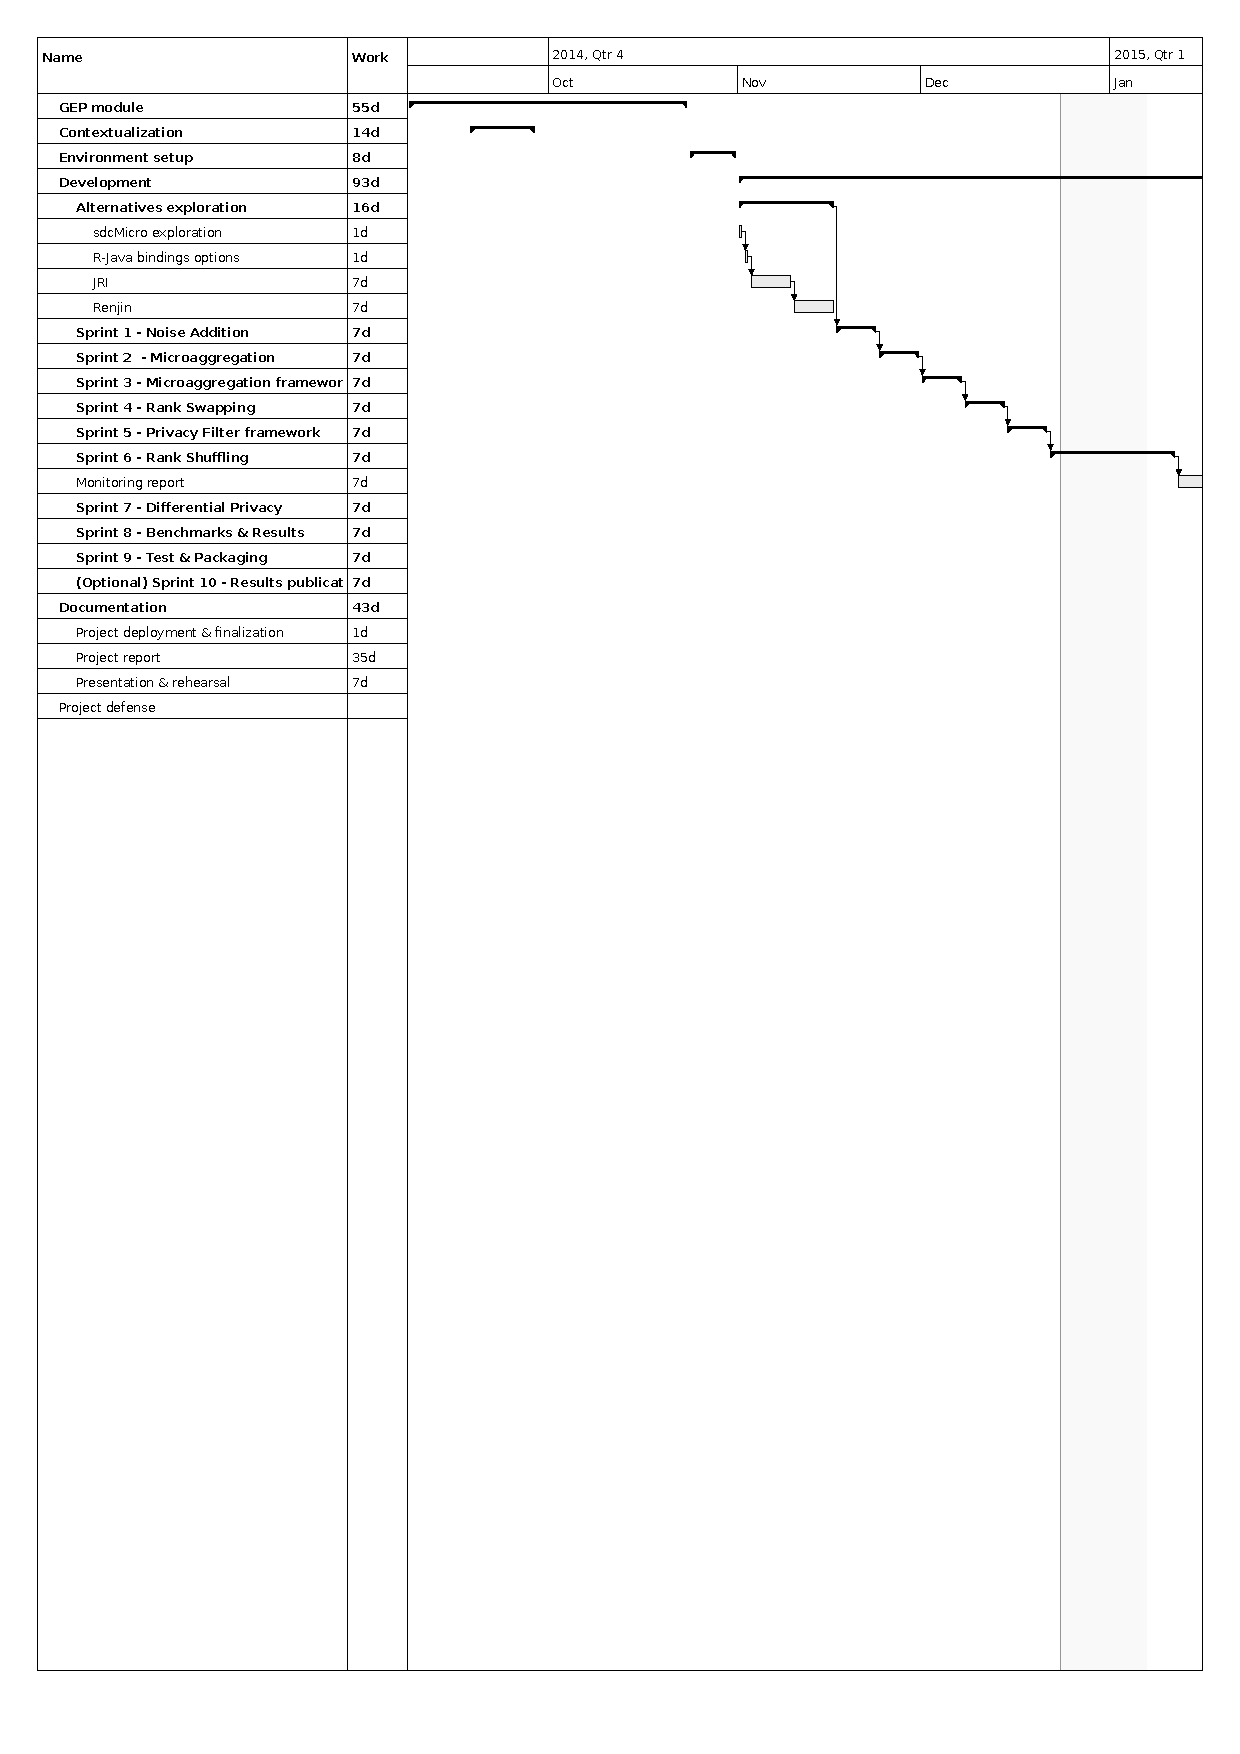
\includepdf[pages={1,2}]{figures/new-gantt-chart.pdf}
